\documentclass[border=5pt]{standalone}
\usepackage{tikz}
\usepackage{xcolor}
\usetikzlibrary{3d,calc,shadows.blur}

% J1 - Blue metallic shaft/axle
\begin{document}
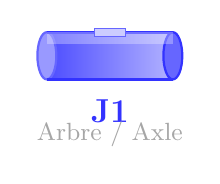
\begin{tikzpicture}

% Shadow
\fill[gray!20,blur shadow={shadow blur steps=5}] (1,0.15) ellipse (0.8 and 0.15);

% Main shaft body (cylinder side)
\fill[left color=blue!70, right color=blue!30, middle color=blue!50]
  (0.2,-0.3) rectangle (1.8,0.3);

% Left end cap (ellipse)
\fill[blue!40] (0.2,0) ellipse (0.12 and 0.3);
\draw[blue!60,thick] (0.2,0) ellipse (0.12 and 0.3);

% Right end cap
\fill[blue!60] (1.8,0) ellipse (0.12 and 0.3);
\draw[blue!80,thick] (1.8,0) ellipse (0.12 and 0.3);

% Outline
\draw[blue!80, line width=1pt] (0.2,-0.3) -- (1.8,-0.3);
\draw[blue!80, line width=1pt] (0.2,0.3) -- (1.8,0.3);

% Highlight
\fill[white,opacity=0.3] (0.2,0.15) rectangle (1.8,0.3);

% Keyway (slot on top)
\fill[blue!20] (0.8,0.25) rectangle (1.2,0.35);
\draw[blue!60] (0.8,0.25) rectangle (1.2,0.35);

% Label
\node[font=\bfseries\large, text=blue!80] at (1.0,-0.7) {J1};
\node[font=\small, text=gray!70] at (1.0,-1.0) {Arbre / Axle};

\end{tikzpicture}
\end{document}
